\section{Original Researcher Choice and Resource-Use Diagnostics}
\label{sec:native-choice-resource}

\subsection{A completed three-control native-choice pilot}
\paragraph{Question and authority.}
The preceding searches did not find a useful structural change. A separate
developer-control study asks whether removing direct agenda assignment and
supplying executable institutional advice exercises the original researcher
choice path. It is not another optimizer run. All three institutions retain
the original four-year world, five founders, 103,107-paper offline corpus,
fixed Qwen3-8B scientists, original T/U measurements and development seed 61001.
Their independently audited cold initial physical-society identities agree.
The known seed is reused; this is neither unused evaluation nor independent
optimizer replication. There are zero designer-generation calls.

The first control is the existing strong post-funding-cost institution with
core-topic agenda assignment. The second cuts that existing project-assignment
actuation and leaves topic choice to the original native researcher routine,
which permits core and related topics. The third adds a code-defined
information office and an addressed context receiver: two nodes and two edges.
Its actual sandboxed code recommends the shortest original eligible duration,
with lexical topic tie-breaking. The host does not force that recommendation,
change original durations or introduce a new topic-assignment API. A larger
nominal choice set is not evidence that a researcher uses it effectively.

\begin{table}[t]
\centering\small
\begin{tabular}{lrrrr}
\toprule
Developer control & $L_T$ & $L_U$ & Project effects & Direction requests \\
\midrule
Direct core assignment & $-20$ & $-15.33$ & 10 & 0 \\
Original native choice & $-14$ & $-10$ & 0 & 10 \\
Native choice with advice & $-16$ & $-12$ & 0 & 10 \\
\bottomrule
\end{tabular}
\caption{Every scheduled control completes. Smaller losses are better; the
first utility is rounded from $-15.333333333333332$. Advice improves both losses
by 2 relative to unadvised choice, but loses to direct assignment. These hand
controls do not establish a newly invented policy, an expected advantage or a
global optimum. Both T and U prefer the same control in this finite set.}
\label{tab:original-choice-controls}
\end{table}

\begin{figure}[t]
\centering
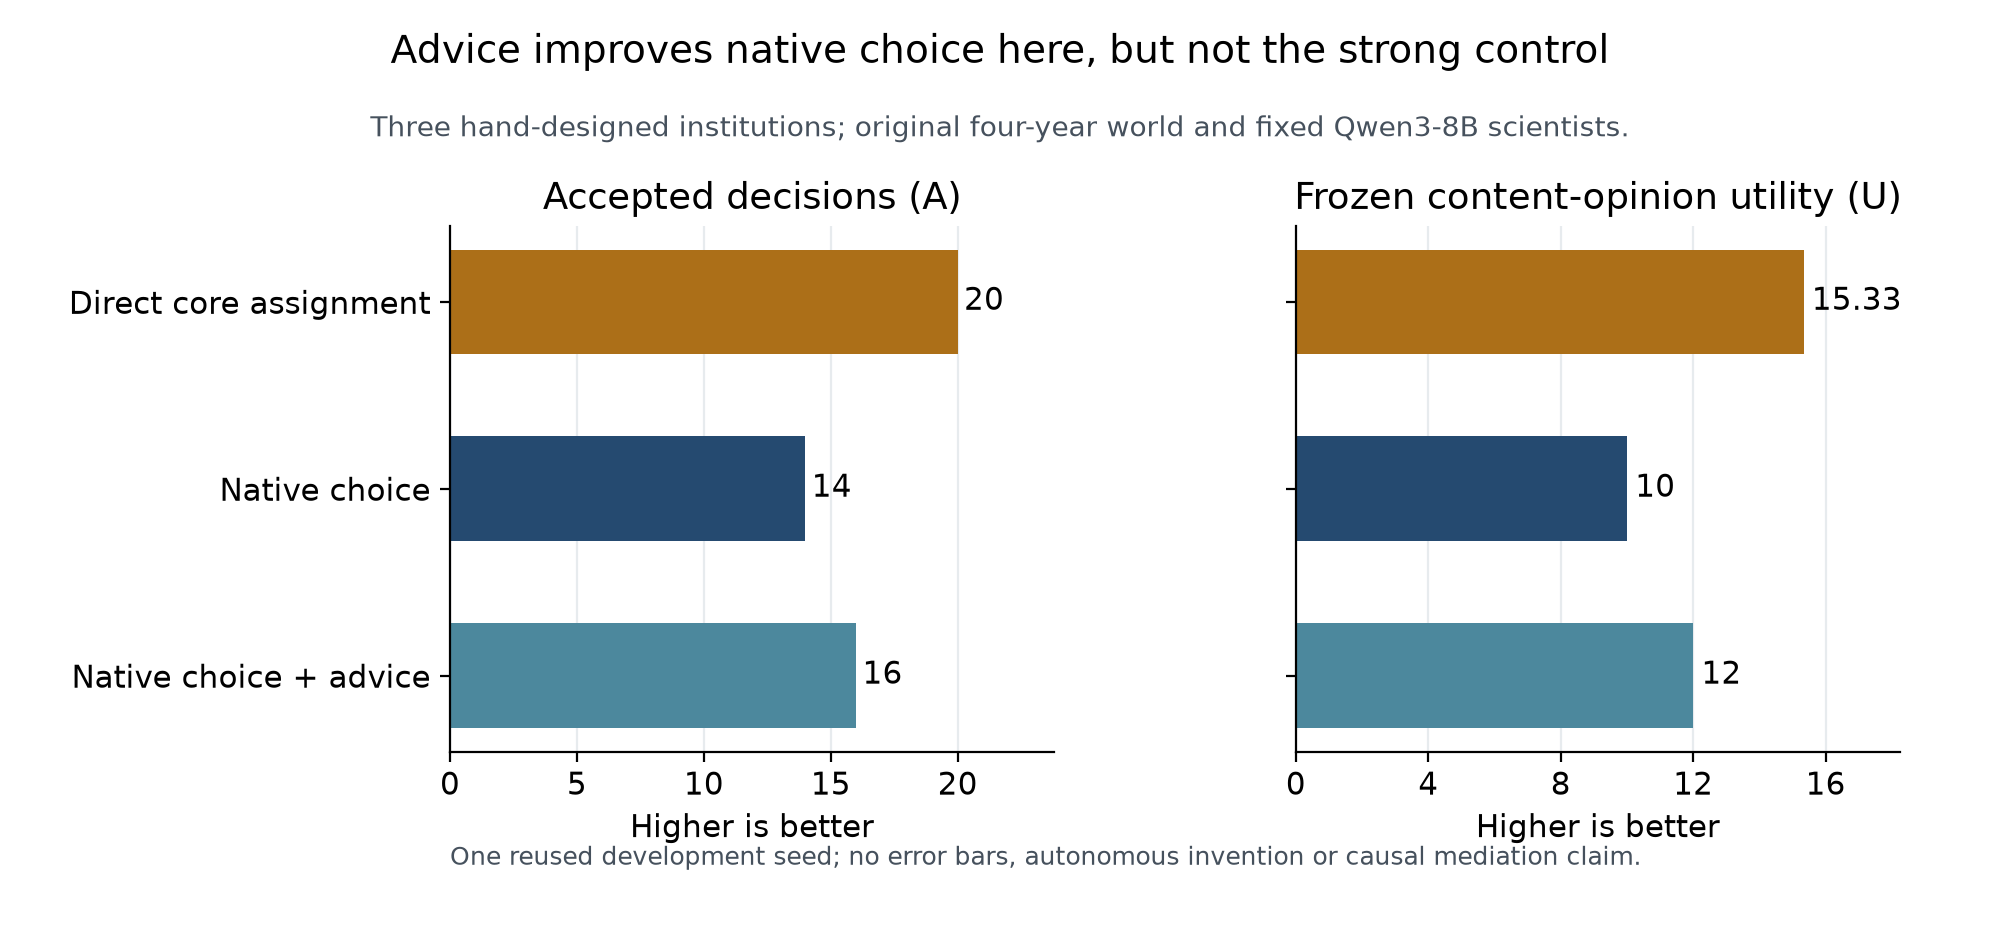
\includegraphics[width=\linewidth]{figures/native-choice-controls-print-v1/native-choice-outcomes.png}
\caption{Actual output and fixed content-opinion utility for the three
completed controls; both are plotted positively, unlike their negative losses
in Table~\ref{tab:original-choice-controls}. One coupled condition supplies no
independent error bars. Neither information delivery nor improvement over an
unadvised control establishes superiority over direct assignment.}
\label{fig:original-choice-controls}
\end{figure}

\paragraph{Advice delivery, topic choice and calendar are different observations.}
All ten advised direction inputs contain current-year advice; ten addressed
messages are stored. Exact recommended-topic matches are 0/10, whereas matches
to the recommended minimum duration are 2/10. The text asks researchers to
consider a topic, not obey a mandatory command, so exact mismatch does not
establish general disobedience. Both unforced conditions make ten native
direction requests with uniquely matched saved direction memories and no host
project-assignment effects. Their full scientist input sequences differ from
each other and from direct assignment.

\begin{table}[t]
\centering\small
\begin{tabular}{lrrr}
\toprule
Original-choice condition & One-year choices & Two-year choices & Three-year choices \\
\midrule
Native choice & 0 & 4 & 6 \\
Native choice with advice & 0 & 6 & 4 \\
\bottomrule
\end{tabular}
\caption{Original catalog durations of the ten observed direction requests
per condition. These are events along two evolving trajectories, not twenty
independent randomized researcher trials. A topic change can change later
request timing, so the two rows do not identify duration-only mediation.}
\label{tab:original-choice-durations}
\end{table}

No one-year topic is selected. All twenty observed selections occur in the
displayed candidate table, but their submitted topic schemas are unrestricted
strings without a topic enum. An enum-forced explanation is therefore not
supported for these actual requests; this is not proof of absence of every
restriction or an identified cause of the choices. The initial actor ending
0002 changes from three-year \code{formal\_methods} to two-year
\code{performance\_analysis}; subsequent calendars also differ. Other altered
information and choices prevent attributing the output difference solely to
this actor or to duration.

Native choice and advised choice share six accepted year/paper/content
occurrences. Eight are native-only and ten are advice-only. Fixed retained
critic opinions give utility totals 10 and 12: the difference of 2 is not
simply the same fourteen records plus two more. Relative to direct assignment,
native choice shares three occurrences and advised choice shares four, with
the remaining content different. This is exact record decomposition, not a
scientific-truth measure or isolated causal estimate of the advice mechanism.

\paragraph{Completion and inference costs.}
The real pilot closes normally in 34m37.04s on the shared host. It records
386 completed scientist responses (127/127/132 by control), 120 separate physical
common-observer POSTs with known terminal attempts, and three empty scientist
load attempts. Scientist usage is 467,505 prompt plus 40,304 completion tokens,
507,809 total; 97,796 cached prompt tokens are a subset, not extra tokens.
There are no wire-only scientist reply gaps. Observer durations are nested
inside elapsed time and not added again. These are provider counts, not FLOPs,
energy, monetary cost or a dedicated machine benchmark. Two original-source
audits and cost exports match, as do all nine paired choice/request/effect
readout files. Readout agreement is reconstruction, not repeated inference.

\subsection{Collected activity resources in the original world}
\paragraph{A passive, prospective-capable instrument.}
Inference costs above are distinct from resources inside the researcher world.
An additive native measurement adapter now reconstructs collected scientific
activity costs from year 0 and every declared annual checkpoint:
\begin{equation}
 K=\sum_{y=1}^{Y}\sum_{a\in\mathcal A_y}
 \left(c^{\mathrm{research}}_{ay}+c^{\mathrm{production}}_{ay}
       +c^{\mathrm{resubmission}}_{ay}+c^{\mathrm{application}}_{ay}\right).
 \label{eq:native-collected-cost}
\end{equation}
Here $\mathcal A_y$ contains every accounted native author, including inactive
actors and later entrants. The terms are actual collected ledger costs, not
requested charges or an active-count approximation. Grant/industry income and
both sides of institutional transfers are excluded: reallocating resources
does not consume them. Requested but uncollected activity costs are reported
separately and are never imputed as collected consumption or made a veto.
Units are model-internal resources, not national expenditure, compute or welfare.

The instrument checks the complete declared horizon, fixed system/world
contract, literal annual actors, cumulative ledger prefixes and between-year
balances, then invokes the native closed-year ledger reconciler. A complete
known empty ledger can measure zero. Missing or inconsistent ledgers and partial
runs have unknown cost, not zero or a numerical penalty. Live and cold paths
append metrics without altering existing measurements, researchers, RNG or raw
files. The existing public native loss/observation boundary accepts the additive
adapter; software checks use scripted models/corpus, not new scientific runs.

\begin{table}[t]
\centering\small
\begin{tabular}{llrr}
\toprule
Closed development study & Observed system(s) & $A$ & $K$ \\
\midrule
Longitudinal & R7 and all ten valid own policies & 18 & 190 \\
Longitudinal & Strong hand control & 20 & 200 \\
Choice pilot & Direct core assignment & 20 & 200 \\
Choice pilot & Original native choice & 14 & 200 \\
Choice pilot & Native choice with advice & 16 & 200 \\
\bottomrule
\end{tabular}
\caption{New retrospective resource measurements, not a new objective-driven
search. The two failed longitudinal proposals keep unknown K. All measured
activity-uncollected costs are zero. The studies remain separate; coincident
points do not represent independent optimizer replications.}
\label{tab:native-collected-cost}
\end{table}

\begin{figure}[t]
\centering
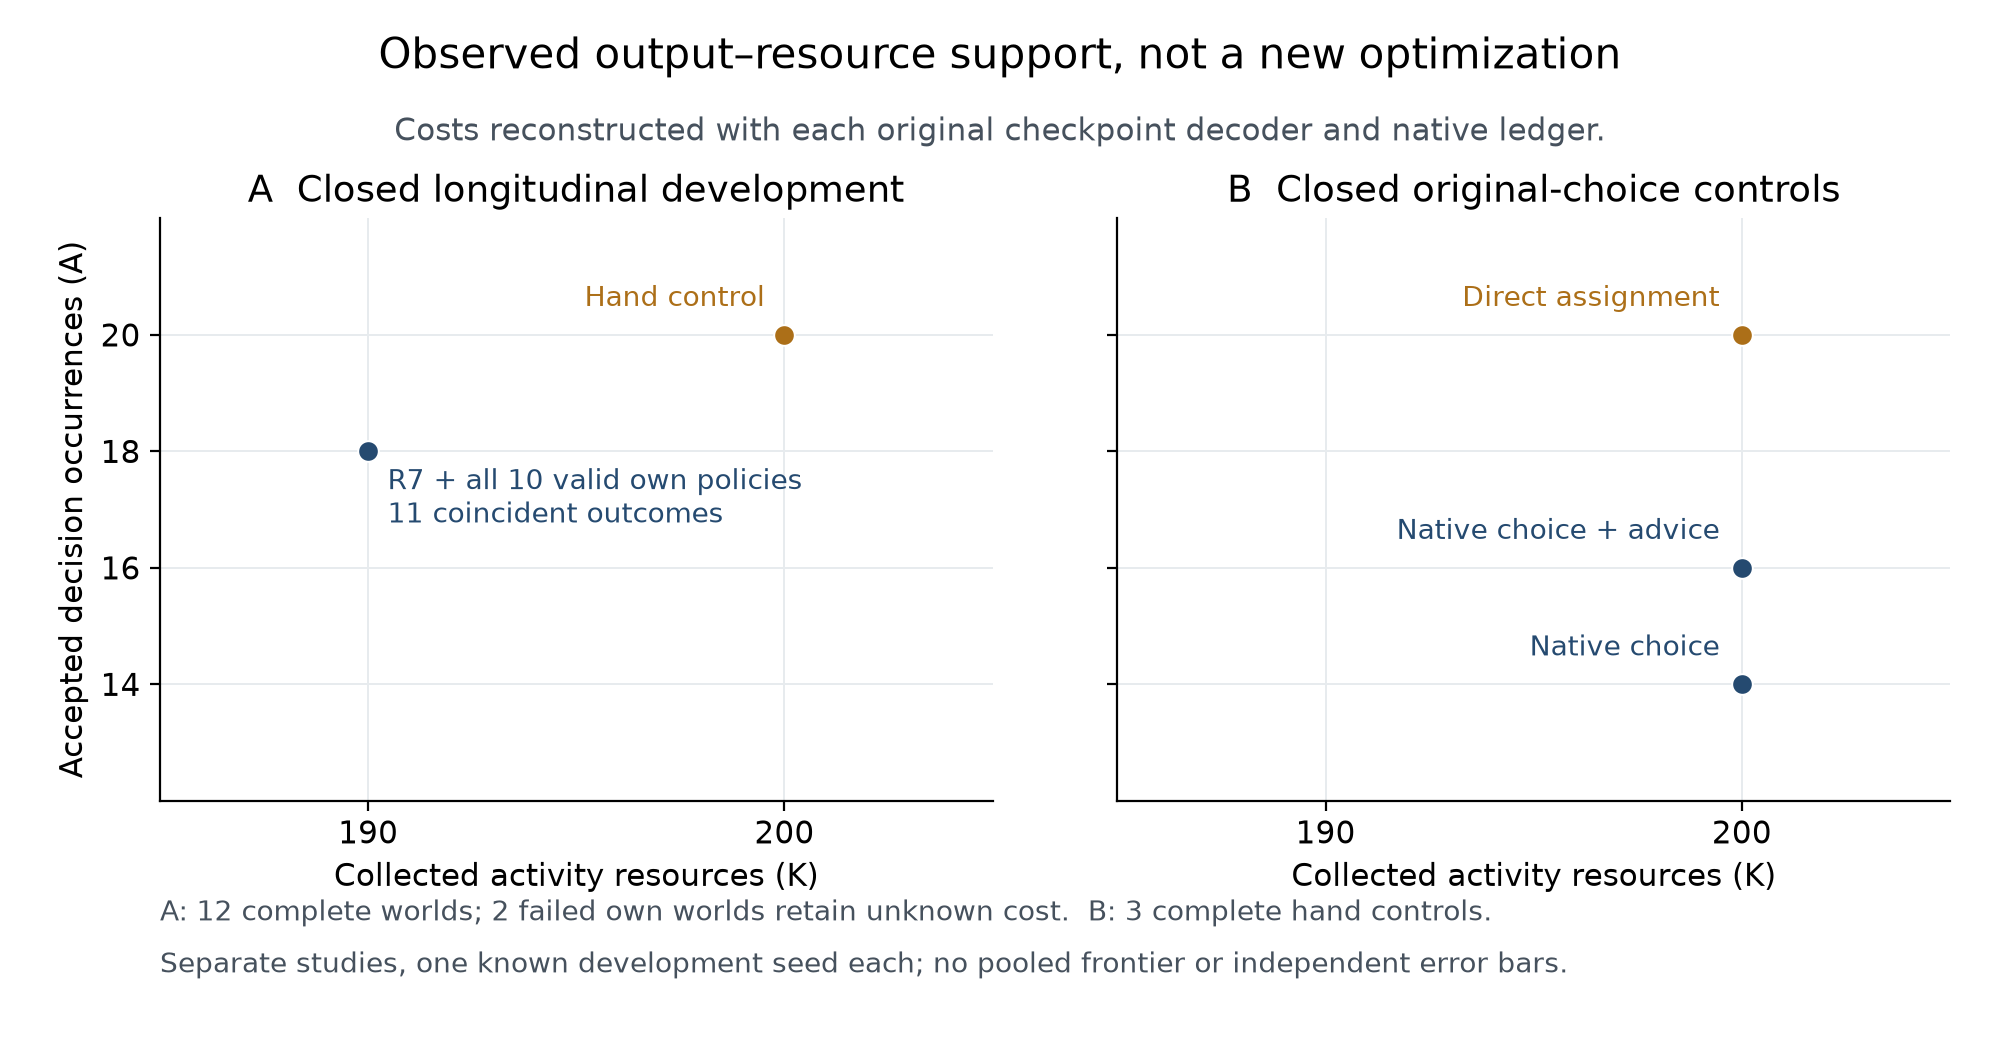
\includegraphics[width=\linewidth]{figures/native-resource-support-v1/output-resource-support.png}
\caption{Separate observed output--resource supports. The longitudinal
reference and ten valid own worlds coincide at $(K,A)=(190,18)$; its hand
comparison is at $(200,20)$. Every choice-pilot world consumes 200. No pooled
or expected frontier, independent error bars or new optimized design is inferred.}
\label{fig:native-collected-cost}
\end{figure}

\paragraph{What the new measurement does and does not change.}
Two byte-identical cold exports per study use the original scientific
checkpoint decoder and resource-ledger reconciler with matching original audits,
fixed scientific sources and unchanged complete raw inventories. Twelve of
fourteen longitudinal worlds measure; two remain unknown. All three choice
controls measure. No new model call, native scientific world or institutional
code execution is performed, and unused evaluation is not newly rescored.

Unlike the observed T/U matrix, the fixed longitudinal R7/hand pair trades
output against resource consumption. A hypothetical new loss
$L_{T,K}=-A+\lambda K$ has equal values for that pair at
$\lambda=(20-18)/(200-190)=1/5$, in accepted decisions per native resource unit.
This algebra does not adopt that weight, validate a policy objective, find a
global frontier or show optimization under a new loss. Neither T/U nor their
historical selections are changed. A new objective-conditioned search would
need its own declared meaning, instrument, same-authority strong comparisons,
finite budget and selection-fixed fresh evaluation. Resource-saving attrition
and other undesirable consequences must remain visible rather than being
removed with an undeclared fairness or improvement filter.
